%% Appendix: DomainBed external example (MedIA revision, v2 pipeline).
%% Every number below is read from results/v2/external/:
%%   domainbed_tables.csv      837 parsed cells (mean +- SE), with source line numbers
%%   domainbed_icc.csv         one row per dataset x selection rule x algorithm
%%   domainbed_provenance.json source URL, checksums, SE convention, caveats
%%   domainbed_icc_training_domain.tex  ERM rows (training-domain validation)
%% produced by `python src/v2/analyze_v2.py domainbed` (parse_domainbed,
%% analyse_domainbed). Table summaries (medians, ranges, CI widths) are computed
%% from domainbed_icc.csv, selection == training_domain, columns code_*.
%% Source: arXiv e-print 2007.01434 (v1), sha256 c76db545...e93081d;
%% paper.tex sha256 7451178f...17bf, appendix tables at lines 935--1381.
%% Figure: figs/fig_domainbed.pdf from src/v2/make_figures_v2.py (S2).
\section{External example: the variance decomposition on DomainBed}
\label{app:domainbed}

To give the ICC of Section~\ref{M-sec:protocol-variance} a reference point
outside pathology, we apply the same estimators to the published
per-environment results of DomainBed \citep{gulrajani2021domainbed}. DomainBed
also evaluates by leave-one-environment-out, so each environment is the test
environment of one fold, as in our design.

\paragraph{Source} We cite the ICLR 2021 version of the paper. The
per-environment tables, however, are taken from the appendix ``Domain
generalization accuracies per algorithm, dataset, and domain'' of the first
arXiv e-print (arXiv:2007.01434v1). It is the only version whose source arXiv
provides, and it reports nine algorithms: ERM, IRM, DRO, Mixup, MLDG, CORAL,
MMD, DANN and C-DANN. The appendix has one table for each of seven datasets
and three model-selection rules, with 837 cells of the form mean $\pm$
standard error (SE). A script parses all of them and stores each with its
source line. Accuracies are in percentage points (pp), rounded to 0.1. In the
Colored MNIST table for training-domain validation the two adversarial
algorithms are named ADA and CondADA, while every other table names them DANN
and C-DANN. We treat them as the same algorithms. The means of the ADA and
CondADA rows over the three environments are 51.5 and 51.9, which are the
Colored MNIST entries of DANN and C-DANN in the main results table of the same
e-print.

\paragraph{From standard errors to standard deviations} Each cell is the mean
over three trials, and each trial repeats the whole study with new random
hyperparameters, weight initializations and dataset splits. The paper does not
give the formula for its SE. We take it from the first public release of the
DomainBed code (commit 8ff97a7), in which \texttt{collect\_results.format\_mean}
computes the population SD (divisor $n$) of the trial accuracies divided by
$\sqrt n$. We assume that the paper's tables were produced with this function.
The sample SD (divisor $n-1$) of a cell with $n=3$ trials is then
\begin{equation}
  s=\mathrm{SE}\cdot\frac{n}{\sqrt{n-1}} .
  \label{eq:domainbed-sd}
\end{equation}
The textbook convention $s=\mathrm{SE}\cdot\sqrt n$ gives SDs smaller by a
factor $\sqrt{(n-1)/n}$, and hence larger ICCs. We report it only as a
sensitivity check. An SE printed as 0.0 is below 0.05 and is used as zero.

\paragraph{Model} For each algorithm and dataset under training-domain
validation (the first rule in DomainBed's main results table, and our primary
rule), we fit model
\eqref{M-eq:oneway} to the test accuracy $y_{ts}$ of held-out environment $t$
in trial $s$. This gives 63 fits, with $K$ between 3 and 6 environments and
$n=3$ trials each. The published summaries are a mean and an SE per cell, so
trials can only be treated as nested within environments, and no crossed trial
effect can be fitted. All estimators of Section~\ref{M-sec:protocol-variance}
depend on the data only through the cell means and the within-cell sums of
squares. We therefore reconstruct three pseudo-observations per cell that
reproduce the published mean and the SD of \eqref{eq:domainbed-sd}. The
analysis of these pseudo-data is exact. With $n=3$ trials in every cell, the
data are balanced and the ICC interval \eqref{eq:iccci} is exact. As a
check, we also compute the grid posterior \eqref{eq:posterior} with
half-Cauchy (scale 10~pp) and half-normal (scale 25~pp) priors on both SDs.

\begin{table}[width=\linewidth,pos=t]
\caption{ICC(1) of test accuracy in DomainBed under training-domain validation,
summarized over the nine algorithms of each dataset (arXiv:2007.01434v1,
appendix tables; three trials per cell; SD from SE by
\eqref{eq:domainbed-sd}). ICC: median and range over algorithms, with the
algorithm with the lowest ICC. CI width: median and range of the width of the
exact 95\% interval \eqref{eq:iccci}. Lower $<0.5$: number of algorithms whose
interval has a lower limit below 0.5. $\hat\sigma_{\text{env}}$ and
$\hat\sigma_{\text{run}}$: medians over algorithms of the between-environment
and between-trial SDs, in pp. SE $=0.0$: cells printed with an SE of 0.0,
out of the dataset's cells under this rule.}
\label{tab:domainbed}
\footnotesize
\begin{tabular*}{\tblwidth}{@{\extracolsep{\fill}}lrrrrlrrr@{}}
\toprule
Dataset & $K$ & SE $=0.0$ & \multicolumn{2}{c}{ICC} & Lowest & CI width & Lower $<0.5$
  & $\hat\sigma_{\text{env}}$\,/\,$\hat\sigma_{\text{run}}$ \\
\cmidrule(lr){4-5}
 & & & median & range & & median (range) & & \\
\midrule
Colored MNIST  & 3 & 5/27  & 1.00 & 1.00--1.00 & DANN   & $<0.01$ ($<0.01$--$<0.01$) & 0 & 36.1\,/\,0.5 \\
Rotated MNIST  & 6 & 23/54 & 0.97 & 0.87--0.99 & C-DANN & 0.09 (0.04--0.37) & 0 & 1.5\,/\,0.3 \\
VLCS           & 4 & 0/36  & 0.99 & 0.96--0.99 & MMD    & 0.07 (0.04--0.19) & 0 & 14.4\,/\,1.8 \\
PACS           & 4 & 2/36  & 0.96 & 0.84--0.99 & C-DANN & 0.20 (0.06--0.58) & 2 & 9.5\,/\,2.1 \\
Office-Home    & 4 & 0/36  & 0.99 & 0.97--0.99 & IRM    & 0.05 (0.03--0.15) & 0 & 11.5\,/\,1.1 \\
TerraIncognita & 4 & 0/36  & 0.77 & 0.51--0.95 & MMD    & 0.72 (0.22--0.95) & 6 & 7.5\,/\,4.0 \\
DomainNet      & 6 & 2/54  & 1.00 & 0.91--1.00 & IRM    & 0.01 (0.01--0.29) & 0 & 19.3\,/\,1.2 \\
\bottomrule
\end{tabular*}
\end{table}

\begin{figure}[pos=t]
\centering
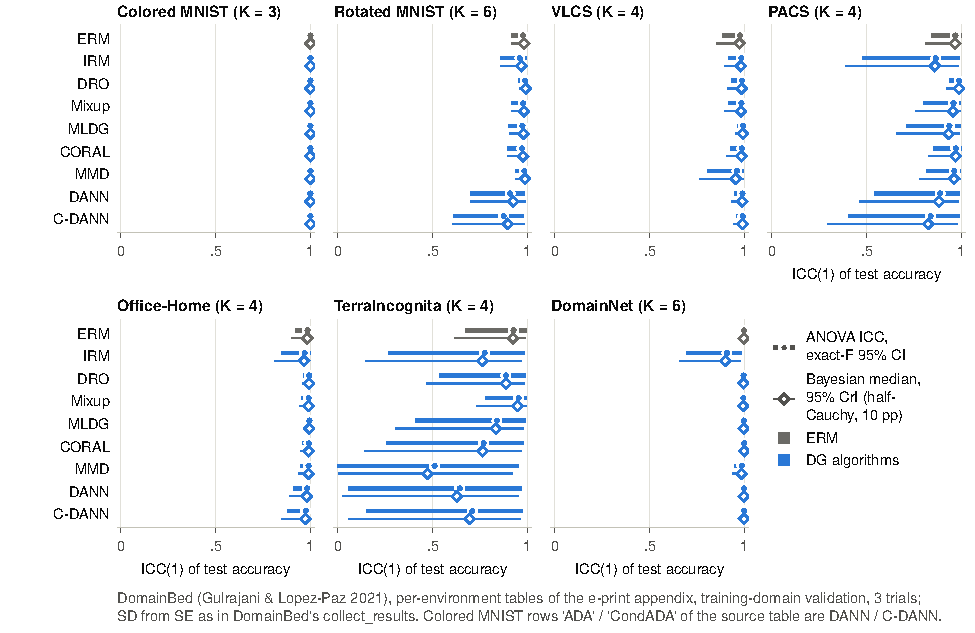
\includegraphics[width=\linewidth]{figs/fig_domainbed}
\caption{ICC(1) of test accuracy for the nine DomainBed algorithms on seven
datasets under training-domain validation (arXiv:2007.01434v1, appendix
tables; three trials per cell; SD from SE by \eqref{eq:domainbed-sd}). Filled
circles and thick bars: ANOVA estimate and exact 95\% interval
\eqref{eq:iccci}. Open diamonds and thin bars: posterior median and
equal-tailed 95\% credible interval under half-Cauchy priors (scale 10~pp).
ERM is shown in gray, the domain-generalization algorithms in blue. The
Colored MNIST rows ADA and CondADA of the source table are shown as DANN and
C-DANN.}
\label{fig:domainbed}
\end{figure}

\paragraph{Results} Table~\ref{tab:domainbed} and Fig.~\ref{fig:domainbed}
summarize the 63 fits. No dataset is run-dominated. The median ICC over the
63 fits is 0.98, and the ICC exceeds 0.8 in all 54 fits outside
TerraIncognita. Colored MNIST, DomainNet, Office-Home and VLCS are the most
strongly environment-dominated (median ICC above 0.98, median interval width
below 0.08). On Colored MNIST, every algorithm reaches 10.0--10.5\%
accuracy on the environment labeled 0.9 in the source table and
71.4--73.3\% on the other two, and the median $\hat\sigma_{\text{env}}$ is
36.1~pp against a median $\hat\sigma_{\text{run}}$ of 0.5~pp. Rotated MNIST
has the smallest spread between environments (median 1.5~pp), but its
between-trial SD is smaller still (0.3~pp). This dataset also has the most SEs
printed as 0.0 (23 of 54 cells), so rounding probably understates its run
variance and overstates its ICC. On PACS the median ICC is 0.96, but two
algorithms (IRM and C-DANN) have intervals that reach below 0.5.
TerraIncognita is the exception. Its median ICC is 0.77, its median
$\hat\sigma_{\text{run}}$ (4.0~pp) is about half its median
$\hat\sigma_{\text{env}}$ (7.5~pp), and six of its nine algorithms have
intervals with lower limits below 0.5. For MMD, the ICC is 0.51 with interval
$[0.00,0.95]$, and the $F$ test of no environment effect gives $p=0.048$.
ERM has ICC 0.93 $[0.67,0.99]$ there. With four environments, the exact interval has
3 numerator degrees of freedom, and on TerraIncognita the median width is
0.72. The Bayesian medians are close to the ANOVA estimates (median 0.76 on
TerraIncognita).

These conclusions do not depend on the SE convention. With the textbook
convention $s=\mathrm{SE}\sqrt n$, the median ICC on TerraIncognita is 0.84
and five fits, rather than eight, have lower limits below 0.5. They do depend
on the selection rule. Under leave-one-domain-out validation, 17 of the 63
fits have lower limits below 0.5, compared with 8 under training-domain
validation and 1 under test-domain (oracle) validation. One example is DANN on
Rotated MNIST, whose three trials disagree so strongly
($\hat\sigma_{\text{run}}=15.0$~pp) that its ICC is 0.00.

\paragraph{Implications for single-environment reporting} Under
training-domain validation, most of the variance of a single DomainBed run is
due to which environment is held out. On six of the seven datasets, the median over
algorithms of the ratio $\hat\sigma_{\text{env}}/\hat\sigma_{\text{run}}$
is between 4.8 and 73.5, and on TerraIncognita it is 1.9. A result on one held-out
environment therefore describes mainly that environment. On these six
datasets the spread between environments is several times the trial-to-trial
SD, so a single environment cannot stand in for the dataset. This is a reason to evaluate on
every environment, as DomainBed does, and to report the worst environment and
the spread over environments together with the mean. On TerraIncognita, the
trial-to-trial SD is a large fraction of the spread between environments, so a
single trial says little about a given environment, even though each trial
already includes a fresh hyperparameter search. Replicating trials is
necessary there, not optional. A high ICC does not show that one algorithm
beats another in every environment. That question concerns the paired
difference \eqref{M-eq:diffvar}, whose variance excludes the shared environment
effect. DomainBed's trials also differ from our seeds. A DomainBed trial
redraws the hyperparameters and the data split, whereas our seeds keep both
fixed within a fold (Section~\ref{M-sec:protocol-lodo}). The two ICCs are
therefore not on the same scale. The comparison shows only that the ICC can be
computed from what a benchmark already publishes, and that its value, and how
precisely it is known, varies with the dataset, the number of environments and
the selection rule.
